
    \cleardoublepage
    \thispagestyle{empty}
    \refstepcounter{chapter} % incrementa o contador
    %\chapter*{Apêndice~\thechapter\\[1ex]Questionário de pesquisa}   
    \vspace*{\fill}
    \begin{center}
        {\bfseries APÊNDICE~\thechapter{ -- }Abreviaturas dos meses do ano}
    \end{center}
    \vspace*{\fill}
    \addcontentsline{toc}{chapter}{APÊNDICE~\thechapter{ -- } Abreviaturas dos meses do ano}
    
%\chapter{Abreviaturas dos meses do ano}\label{cap:apendicec}
\newpage

%\centerline{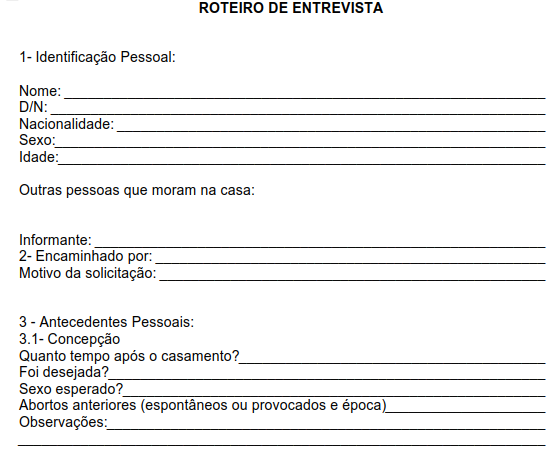
\includegraphics[width=\textwidth]{./PosTexto/Ilustracoes/roteiro}}%% Imagem (Dimensões e localização)

\begin{center}
\textbf{Abreviaturas dos meses do ano}    
\end{center}


\doublespacing{

\begin{tabular}{l l}
Janeiro –  &  jan. \\
Fevereiro –  & fev. \\
Março –  &mar.\\
Abril –   &abr.\\
Maio –  &maio (único não abreviado).\\
Junho –   &jun. \\
Julho –   &jul.\\
Agosto –  &ago.\\
Setembro –  &set.\\
Outubro –  &out.\\
Novembro –  &nov.\\
Dezembro –  &dez.\\
\end{tabular}
}